\subsection{LuaLetterLizard: Lua Letter Lizard Implementation}
\label{luaimpl}

% Introduce Language
% LUA
%   - shares many similaritise with javascript
%   - minimal but powerful
%   - local variable declared only where needed, "everything is a table"
%   - designed primarily as an extensible extension language
%   - chosen becasuse it is a fast, simple, versitile languages with many advanced 
%     features (eg. operator overloading)
%   - look at Wikipedia and language website for more information

% talk about how this version is implemented (eg classes, etc)
% show screenshots
% talk about implementation: language features that were useful,
% class diagrams, sequence diagrams, snippets of code, etc

% NOTE: NEED TO MENTION HOW TO INSTALL DEPENDENCIES (I.E. LOVE)
%1. http://www.lua.org/about.html
Lua is a light weight programming language designed as a scripting language. Lua is generally described as a 'multi-paradigm' programming language because it provides a small set of extensible features that can be extended to fit various problems rather than providing definite features for a specific paradigms. Lua has a short learning curve and is easy to pick up. Lua has a number of features which endorse its  nature. Lua for example does not support inheritance but allows it to be implemented by using metatables.
Lua provides a fundamental data structure 'table' which can be used to represent everything. Tables are infact the only data structures in Lua and can be used to implement other data structures such as arrays, sets, list, records and other data structures.Lua tables can be used to implement features such as namespaces and classes.Lua shares a lot of similarities with JavaScript. For instance, 'tables' in Lua are quite similar to JavaScript 'objects', the only difference being that in JavaScript objects can be indexed with only string or integer values but Lua tables can be indexed with any value of the language (except nil). 
Lua is dynamically typed and is light enough to fit on any operating system. The Lua interpreter is extremely lightweight, it is only 180 kB when compiled. Hence, Lua is very fast as compared to Python and JavaScript. It is a minimal but powerful language. By including only a minimal set of data types, Lua attempts to strike a balance between power and size \cite{about_lua}
Lua is specifically used in game development because of its speed, portability, embeddable nature and the simple but powerful design. In order to enable embedding in other languages, Lua provides a well documented API to extend programs written in other languages. 
A number of language specific features in Lua are first class functions, dynamic module loading, automatic coercion and closures. Although Lua does not support object oriented concepts of classes and methods, they can be simulated using tables and first class functions. By placing functions and related data into a table, objects are formed. Inheritance can be implemented  using metatables. It is similar to JavaScript in this way as there is no explicit concept of a class in Lua, rather prototypes are used similar to JavaScript and new objects are created by a factory method, i.e, by cloning existing objects. Lua provides 'syntactic sugar' in facilitating object orientation. In order to declare member functions inside a table, the programmer can use \texttt{table:func(args)}. The colon operator adds a hidden 'self' parameter to function calls.
\subsubsection{Lua Game Framework}
The framework used for developing the Lua based implementation of Letter Lizard was done using \textbf{LOVE}. Love is a free, open source framework for building 2D games in Lua. The Love framework has cross platform adaptability and was installed from the Love homepage~\cite{about_love}. To run a game, Love can load a game in two ways, i.e, from a folder that contains a main.lua file or from a .love file that has a main.lua in the root directory. Love utilizes callback functions to perform various tasks. Love provides placeholders for callback function in order to structure the game logic. For instance, \texttt{love.load} function is called only once when the game is started and is usually used to to load resources, initialize variables and set specific settings. \texttt{love.draw} function is where all the drawing happens and if any of the love.graphics.draw objects are called outside of this function, its not going to have any effect. The following images show screenshots from the Lua version of Letter Lizard.

\begin{figure}
    \centering
    \begin{subfigure}{0.49\textwidth}
        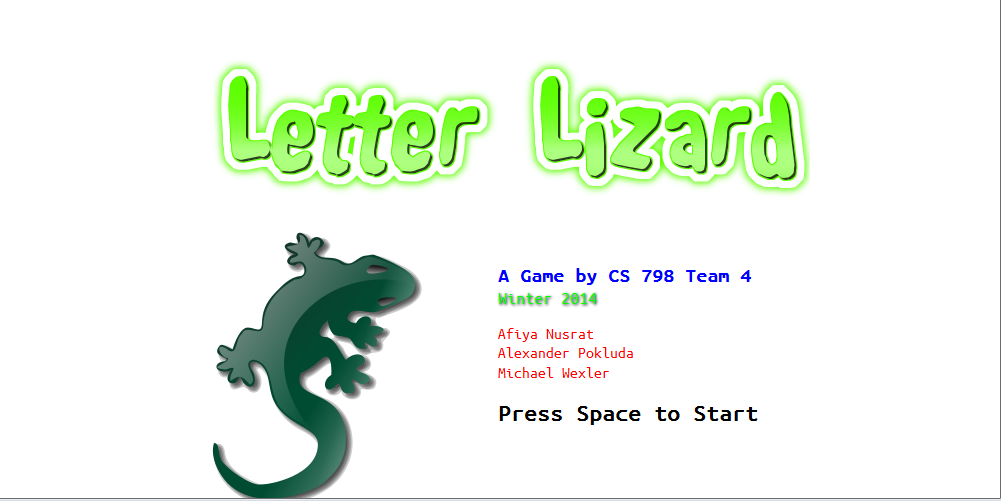
\includegraphics[width=\textwidth]{../screenshots/luasplash.png}
        \caption{LuaLetter Lizard Splash Screen}
        \label{luasplash}
    \end{subfigure}
    \begin{subfigure}{0.49\textwidth}
        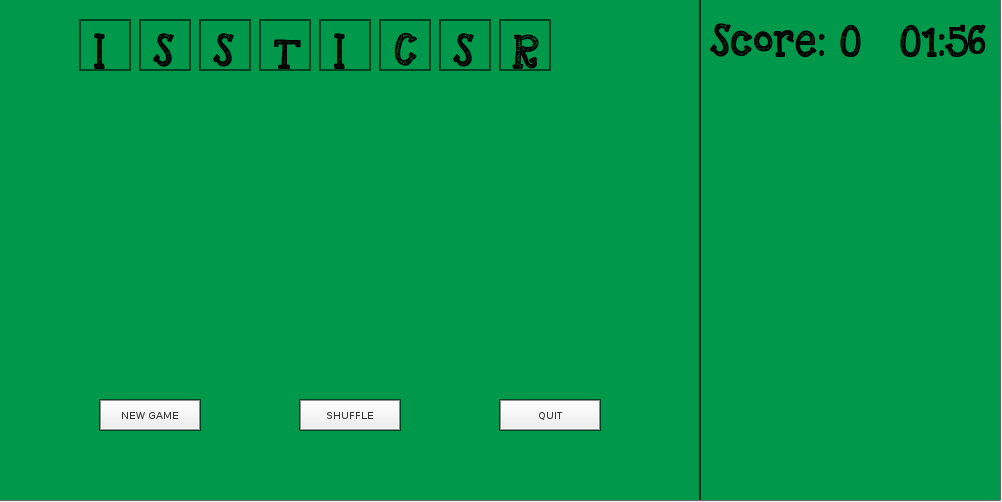
\includegraphics[width=\textwidth]{../screenshots/luabegin.png}
        \caption{Gameplay}
        \label{luabegin}
    \end{subfigure}
    \caption{The Splash screen and the Gameplay screen as viewed in LuaLetter Lizard
    showing (a) the splash screen and (b) the gameplay.}
    \label{luascreenshots1}
\end{figure}

\begin{figure}
    \centering
    \begin{subfigure}{0.49\textwidth}
        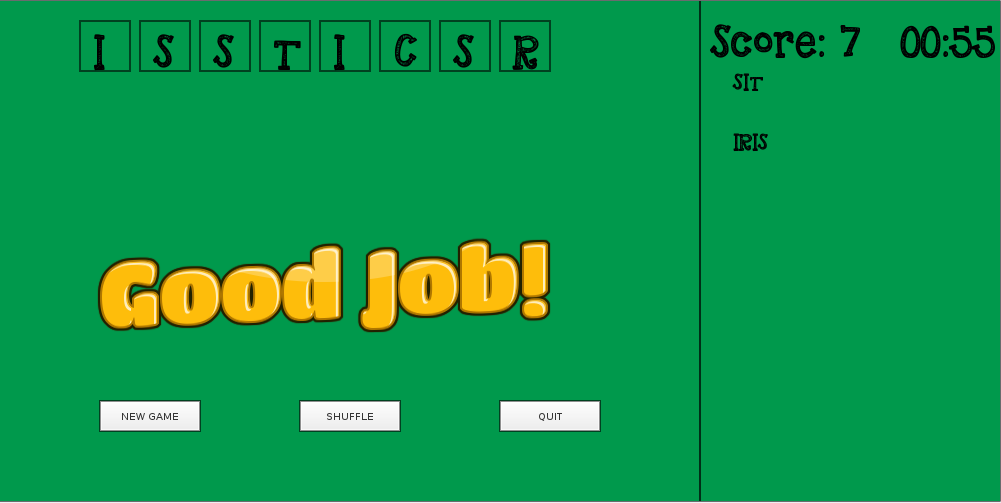
\includegraphics[width=\textwidth]{../screenshots/luagameplay.png}
        \caption{Gameplay Mode}
        \label{luagameplay}
    \end{subfigure}
    \begin{subfigure}{0.49\textwidth}
        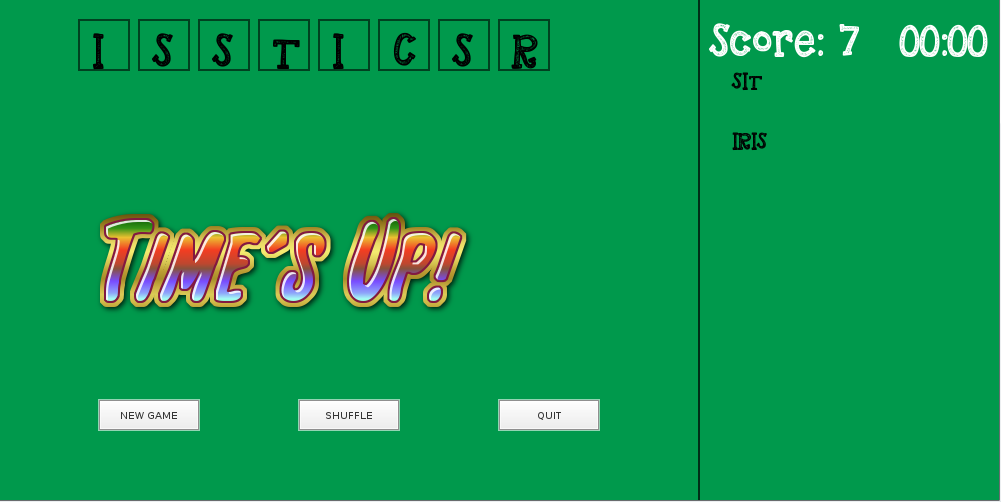
\includegraphics[width=\textwidth]{../screenshots/luagameover.png}
        \caption{Game Over}
        \label{luagameover}
    \end{subfigure}
    \caption{The screens displayed during gameplay begin and gameover.}
    \label{luascreenshots2}
\end{figure}


	The game structure consists of five different Lua modules. These were \texttt{main.lua}, \texttt{conf.lua}, \texttt{games.lua},  \texttt{helper\_functions.lua}, \texttt{gamestate.lua} and \texttt{config.lua}. The \texttt{main.lua} module is the driver of the game and utilizes all the other modules. \texttt{conf.lua} contains game configurations and is run exactly once before \texttt{main.lua} by love.exe. \texttt{games.lua} contains 300 games pre-generated using \texttt{game\_generator.py} module. \texttt{gamestate.lua} was taken from  a small, Lua utility library and enables us to maintain state information within the game and allow us to switch between states. Since Lua is a very low-level language, we had to code a lot of functionality on our own. These free standing functions are contained in the\texttt{helper\_functions.lua} module. \texttt{config.lua} contains additional game configurations which are used by \texttt{main.lua} to drive the game. In order to execute the game we need to run the love.exe file and give the directory containing the main.lua file as an input.
	\subsubsection{Game Logic and Implementation}
	
	The \texttt{main.lua} file contains the main game logic structured within callback functions.In this file, we declare two Lua table structures, menu and game. We implement metatables a powerful feature provided by Lua, to enable the concept of state within the game. Within the menu table we declare functions which are associated with the menu and are called only when menu is the current state of the game. Within the game structure, we declare functions which are called only when the we enter the gameplay mode.
	The menu table contains function which are called when we start the game and the splash screen is loaded. The function \texttt{menu:init()}is called when the game is first loaded into memory and the splash screen is displayed. In order to actually draw the splash screen function \texttt{menu:draw()} is called. Within the \texttt{love.keypressed()} function we check if the player has hit the spacebar, and if true, the state of the game is switched to game and the associated callback functions are then called. All the game play logic is structured within game table. Lua is different from python in a way  that there is no infinite loop which keeps running. Rather, callbacks are called as and when required. Function \texttt{love.update()} is called every frame of the game and it is passed a parameter \texttt{dt} which is the time passed since the last time update was called.
	
\begin{minipage}[t]{1\linewidth}
%\centering
\begin{lstlisting}[language={[5.2]Lua}, %
  title={Splash Screen}, label=splash]
	local menu = {}
	function menu:init()
   		splash = love.graphics.newImage("splash.png")
	end

	function menu:draw()
    	love.graphics.setColor(255,255,255,255)
    	love.graphics.draw(splash, 0 ,0)
	end

\end{lstlisting}
\end{minipage}

Once we enter into the game play mode, the corresponding callback functions defined in the game table are called. For instance in the following code snippet, function \texttt{game:draw()} is called to draw objects onto the screen while we are currently in the gameplay state i.e., the default \texttt{love.draw()} function is overridden. Hence, callbacks defined when in a particular state are called as and when required.


\begin{minipage}[t]{1\linewidth}
%\centering
\begin{lstlisting}[language={[5.2]Lua}, %
  title={Game State}, label=game]
	function game:draw()
    love.graphics.setColor(black)
    love.graphics.line(700,0, 700, 500)
    for i, letter in ipairs(letters_guessed) do
        x = letters_guessed_left + i * square_width + i * spacing
        y = letters_guessed_top
        love.graphics.rectangle("line", x, y ,square_width,square_width)
        love.graphics.setFont(number_fnt_40)
        love.graphics.print(letter, x + square_width/4, y + square_width/5)
    end

\end{lstlisting}
\end{minipage}

In order to maintain state, we utilized an external Lua library, \texttt{hump}. This is a lightweight library with contains helper code for embedding a set of different functionality within our code. Since Lua is very low level, we had to code a lot of functionality ourselves, and using hump minimized a lot of extra work for us considering the time constraints. This was another advantage of using the Love framework, as Love has a very good online community and many of Lua's functionality have been implemented by other Lua game developers and can be utilized under the Open Source License.
Another important part of the game logic is checking for events. For this, we utilized the callback functions defined by Love, \texttt{love.keypressed()} and \texttt{love.mousepressed()}. Within the former callback we check for events that fire when a keyboard key is pressed by the player and define logic for the corresponding action that needs to be taken whereas in the later we check for events when the player click a particular button which fire the corresponding actions. In the following code snippet,
	
\begin{minipage}[t]{1\linewidth}
%\centering
\begin{lstlisting}[language={[5.2]Lua}, %
  title={Keypressed Event}, label=keypressed]
	function menu:keypressed(key)
    if key == ' ' then
        Gamestate.switch(game)
    end
end

\end{lstlisting}
\end{minipage}
we check if the 'space' key has been pressed by the player while we are in state 'menu' and switch game state to 'game' to begin playing the game.
